\documentclass[10pt, landscape]{article}
\usepackage[scaled=0.92]{helvet}
\usepackage{calc}
\usepackage{multicol}
\usepackage{ifthen}
\usepackage[a4paper,margin=5mm,landscape]{geometry}
\usepackage{amsmath,amsthm,amsfonts,amssymb}
\usepackage{color,graphicx,overpic}
\usepackage{hyperref}
\usepackage{newtxtext} 
\usepackage{enumitem}
\usepackage{amssymb}
\usepackage[table]{xcolor}
\usepackage{vwcol}
\usepackage{tikz}
\usetikzlibrary{arrows.meta}
\usetikzlibrary{calc}
\usepackage{mathtools}
\usepackage{nicematrix}
\usepackage[T1]{fontenc} %%% <--- NOTE THIS
% for relations
\usepackage{cancel}
\usepackage{ mathrsfs }
\usepackage{listings}
\setlist{nosep}

\pdfinfo{
  /Title (CS2030S.pdf)
  /Creator (TeX)
  /Producer (pdfTeX 1.40.0)
  /Author (Seamus)
  /Subject (Example)
  /Keywords (pdflatex, latex,pdftex,tex)}

\lstset{language=Java,keywordstyle={\bfseries \color{black}}}

% Turn off header and footer
\pagestyle{empty}

\newenvironment{tightcenter}{%
  \setlength\topsep{0pt}
  \setlength\parskip{0pt}
  \begin{center}
}{%
  \end{center}
}

% redefine section commands to use less space
\makeatletter
\renewcommand{\section}{\@startsection{section}{1}{0mm}%
                                {-1ex plus -.5ex minus -.2ex}%
                                {0.5ex plus .2ex}%x
                                {\normalfont\large\bfseries}}
\renewcommand{\section}{\@startsection{section}{2}{0mm}%
                                {-1explus -.5ex minus -.2ex}%
                                {0.5ex plus .2ex}%
                                {\normalfont\normalsize\bfseries}}
\renewcommand{\subsection}{\@startsection{subsection}{3}{0mm}%
                                {-1ex plus -.5ex minus -.2ex}%
                                {1ex plus .2ex}%
                                {\normalfont\small\bfseries}}%
\renewcommand{\familydefault}{\sfdefault}
\renewcommand\rmdefault{\sfdefault}
% makes nested numbering (e.g. 1.1.1, 1.1.2, etc)
\renewcommand{\labelenumii}{\theenumii}
\renewcommand{\theenumii}{\theenumi.\arabic{enumii}.}
\renewcommand\labelitemii{•}
%  for logical not operator
\renewcommand{\lnot}{\mathord{\sim}}
\renewcommand{\bf}[1]{\textbf{#1}}
\newcommand{\abs}[1]{\vert #1 \vert}
\newcommand{\Mod}[1]{\ \mathrm{mod}\ #1}

\makeatother
\definecolor{myblue}{cmyk}{1,.72,0,.38}
\everymath\expandafter{\the\everymath \color{myblue}}
% Define BibTeX command
\def\BibTeX{{\rm B\kern-.05em{\sc i\kern-.025em b}\kern-.08em
    T\kern-.1667em\lower.7ex\hbox{E}\kern-.125emX}}
\let\iff\leftrightarrow
\let\Iff\Leftrightarrow
\let\then\rightarrow
\let\Then\Rightarrow

% Don't print section numbers
\setcounter{secnumdepth}{0}

\setlength{\parindent}{0pt}
\setlength{\parskip}{0pt plus 0.5ex}
%% this changes all items (enumerate and itemize)
\setlength{\leftmargini}{0.5cm}
\setlength{\leftmarginii}{0.5cm}
\setlist[itemize,1]{leftmargin=2mm,labelindent=1mm,labelsep=1mm}
\setlist[itemize,2]{leftmargin=4mm,labelindent=1mm,labelsep=1mm}

%My Environments
\newtheorem{example}[section]{Example}
% -----------------------------------------------------------------------

\begin{document}
\raggedright
\footnotesize
\begin{multicols*}{4}


% multicol parameters
% These lengths are set only within the two main columns
\setlength{\columnseprule}{0.25pt}
\setlength{\premulticols}{1pt}
\setlength{\postmulticols}{1pt}
\setlength{\multicolsep}{1pt}
\setlength{\columnsep}{2pt}

\begin{center}
    \fbox{%
        \parbox{0.8\linewidth}{\centering \textcolor{black}{
            {\Large\textbf{CS2030S}}
            \\ \normalsize{AY24/25 Sem 1}}
            \\ {\footnotesize \textcolor{myblue}{by ngmh}} 
        }%
    }
\end{center}

\section{Programming Languages}
\begin{itemize}
\item Dynamic v/s Static Typing: Dynamic languages have variables that can hold values of multiple different unrelated types. Static languages have variable types that must be declared and cannot be changed \\
\item Strong v/s Weak Typing: Stronger languages have greater rules in their type system to ensure type safety
\end{itemize}

\section{Tombstone Diagram}
\begin{center}
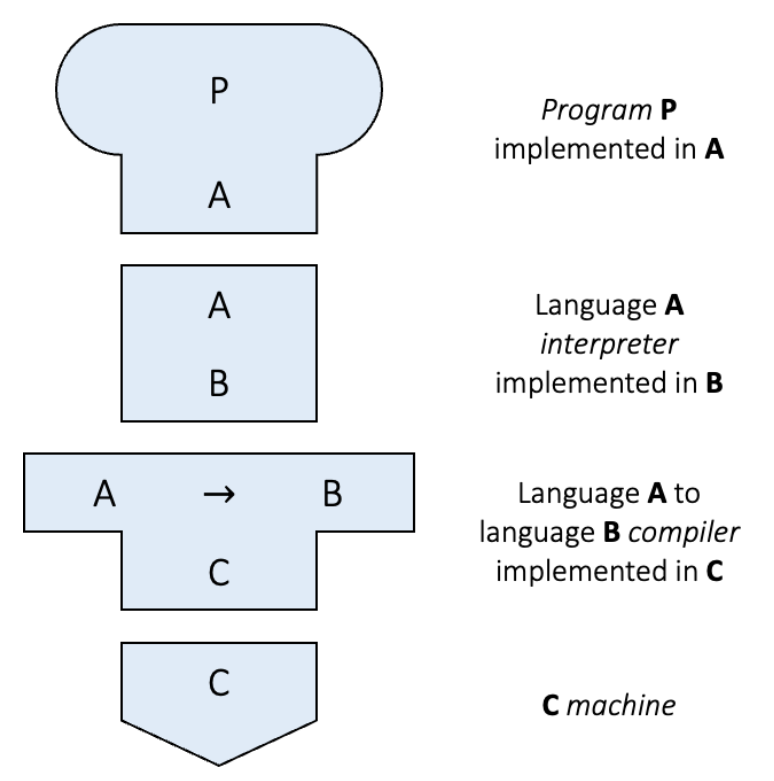
\includegraphics[width=0.7\linewidth]{tombstone.png}
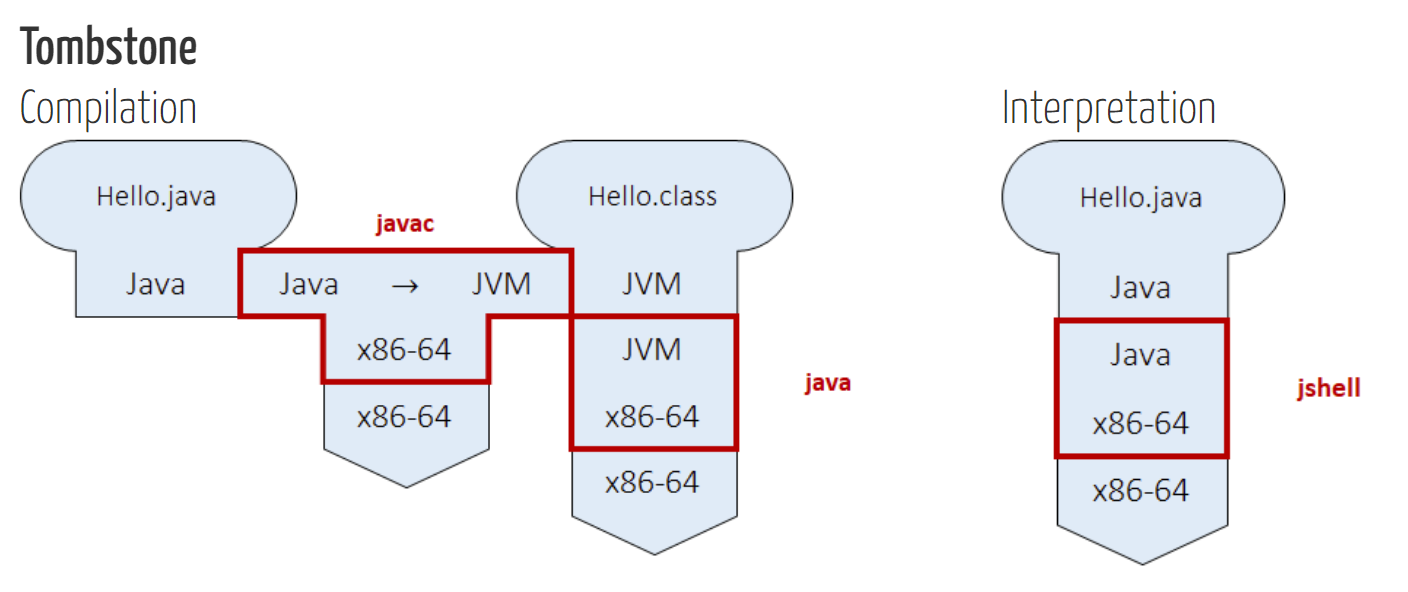
\includegraphics[width=\linewidth]{java.png}
\end{center}

\section{Subtyping}
\begin{itemize}
\item T is a subtype of S (T <: S) if code written for S can be safely used for T \\
\item T has a narrower scope, while S has a wider scope \\
    \begin{itemize}
        \item T can be put into S (widening) \\
        \item S can be explicitly typecast into T (narrowing) \\
    \end{itemize}
\item Properties
\begin{itemize}
    \item Reflexive: T < : T \\
    \item Transitive: T <: S, S <: U, T <: U \\
    \item Anti-Symmetric: If T <: S, S <: T, then S = T
\end{itemize}
\end{itemize}
\section{Primitive Types}
\begin{itemize}
    \item byte <: short <: int <: long <: float <: double \\
    \item char <: int
\end{itemize}

\section{Reference Types}
\begin{itemize}
    \item Anything that is not a Primitive Type such as classes
    \item Stores only a reference to the value
    \item Two reference variables can share the same value like pointers, equality by default compares references not actual value
    \item If uninitialized, have null values and throw errors
\end{itemize}

\section{Class Fields and Methods}
\begin{itemize}
    \item Use the \lstinline{static} keyword to specify
    \item Fields can be accessed using \lstinline{Class.field}, common value shared across the entire class
    \item Methods can also be accessed using \lstinline{Class.method()}, but the \lstinline{this} keyword will \textbf{NOT} work
\end{itemize}

\section{Pillars of OOP}
\begin{itemize}
    \item Encapsulation: Bundle of variables (fields) and functions (methods), by making a \lstinline{class}, that can be represented in a class diagram
    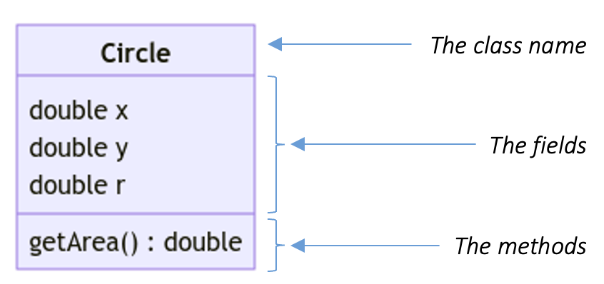
\includegraphics[width=\linewidth]{class.png}
    \item Abstraction: Writing reusable code by grouping sets of instructions
    \item (Not a Pillar) Composition: Creating wrapper class around an object with additional fields, models a \textbf{Has-A} relationship
    \item Inheritance: Preserve methods and fields of the original object, models a \textbf{Is-A} relationship
    \item Polymorphism: Allowing one variable to take on different run-time types, or different methods to be called
\end{itemize}

\section{OOP Style}
\begin{itemize}
    \item Information Hiding:
    \begin{itemize}
        \item Prefer marking fields as \lstinline{private}, unless necessary, to keep abstraction barrier
        \item Private fields can still be accessed by objects of the same class
        \item If absolutely necessary, use a \textbf{getter} or \textbf{setter} to access
    \end{itemize}
    \item Tell Don't Ask: Client should tell the class what to do, rather than gathering information from the class for actions
\end{itemize}

\section{Stack and Heap}
\begin{itemize}
    \item Stack:
        \begin{itemize}
            \item Where all variables are allocated and stored
            \item Contains \textbf{Call Frames}, which are created when methods are invoked and destroyed when methods are returned from
        \end{itemize}
    \item Heap:
        \begin{itemize}
            \item Where objects are allocated and stored
            \item Whenever \lstinline{new} is used, a new object is created on the heap
            \item Objects are stored as Class Name, Instance Fields and Values, and Captured Variables
        \end{itemize}
    \item Example Diagram when \lstinline{move} is called
    \begin{lstlisting}
    class Point {
      private double x;
      private double y;
      public Point(double x, double y) {}
      public double distanceTo(Point q) {}
    }
    Point p1 = new Point(0, 0);
    Point p2 = new Point(1, 1);
    p1.distanceTo(p2);
    \end{lstlisting}
    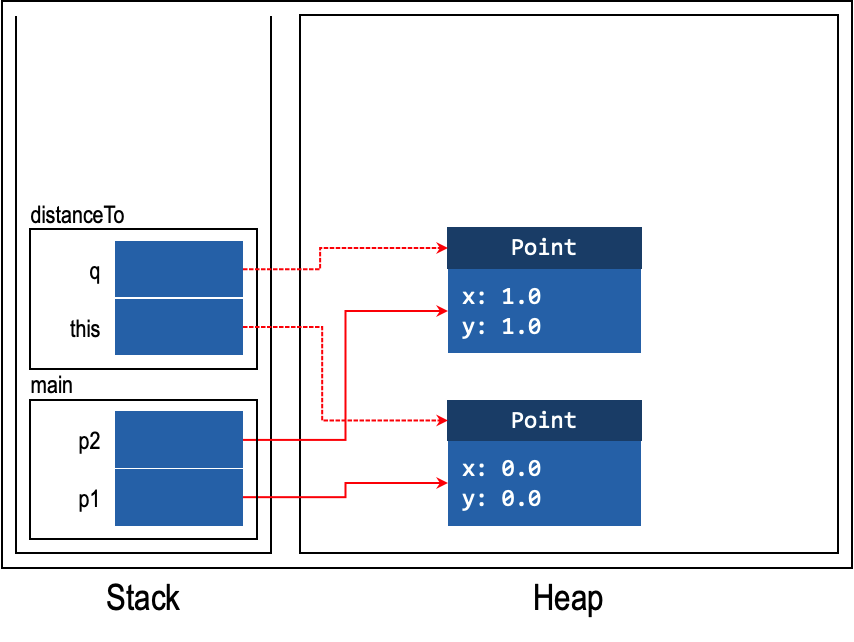
\includegraphics[width=\linewidth]{006b.png}
    \item Example Diagram when \lstinline{distanceTo} is called
    \begin{lstlisting}
    class Point {
      // ...
      public void move(double x, double y) {}
    }
    Point p1 = new Point(0, 0);
    Point p2 = new Point(1, 1);
    double x = 5;
    double y = 5;
    p1.move(x, y);
    \end{lstlisting}
    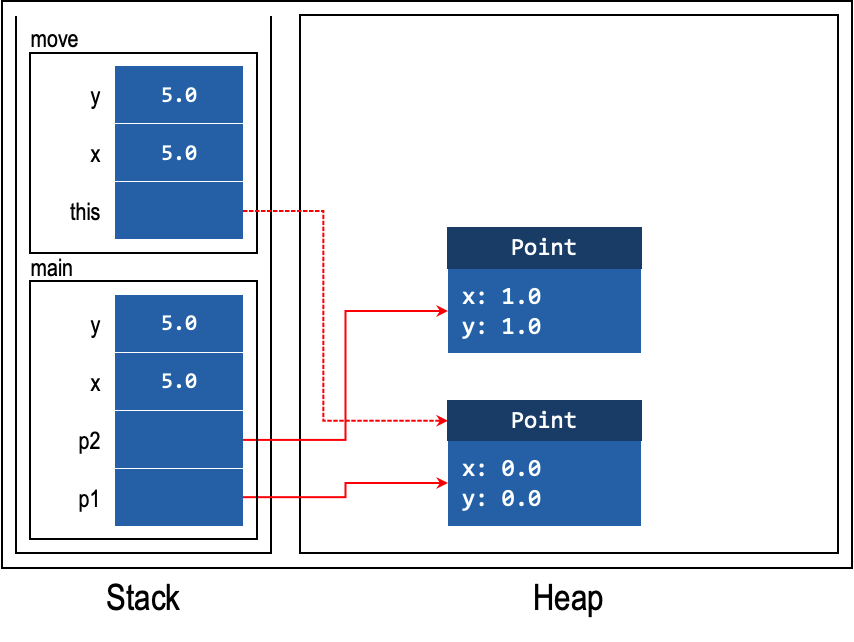
\includegraphics[width=\linewidth]{007c.png}
\end{itemize}

\section{Inheritance}
\begin{itemize}
    \item Use the \lstinline{extends} keyword
    \item Use \lstinline{super()} to call the parent constructor, \textbf{MUST BE FIRST LINE}
    \item Overriding
    \begin{itemize}
        \item Use the \lstinline{@Override} annotation
        \item Must match \textbf{Method Descriptor} (Name of method, Type of Parameters, Return Type)
    \end{itemize}
    \item Overloading
    \begin{itemize}
        \item Method with same name but different \textbf{Method Signature} (Name of method, Type of Parameters)
    \end{itemize}
    \item Liskov Substitution Principle
    \begin{itemize}
        \item Any property of objects of type T should be true for any object of type S where S <: T
        \item Don't break expectations of the parent class
        \item Can use the \lstinline{final} keyword to prevent inheritance of classes, or modification of methods, or re-assignment of fields
    \end{itemize}
\end{itemize}

\section{Dynamic Binding}
\begin{itemize}
    \item Compile Time Type v/s Run Time Type
    \begin{itemize}
        \item \lstinline{Circle c = new ColouredCircle()}
        \item CTT(c) = Circle, RTT(c) = ColouredCircle
    \end{itemize}
    \item Example: \lstinline{obj.foo(arg)}
    \item Compile Time
    \begin{itemize}
        \item Check CTT(obj)
        \item Check CTT(arg)
        \item Find all accessible methods named foo, including those in supertypes of CTT(obj)
        \item Find most specific method (narrowest) that fits with CTT(arg)
        \item Record the method descriptor
    \end{itemize}
    \item Run Time
    \begin{itemize}
        \item Retrieve method descriptor
        \item Determine RTT(obj)
        \item Start from RTT(obj) and find first method fitting descriptor
        \item Recurse upwards until found
    \end{itemize}
    \item Does not apply to Class methods
\end{itemize}

\section{Abstract Classes}
\begin{itemize}
    \item A general class, that should \textbf{NEVER} be instantiated
    \item Use the \lstinline{abstract} keyword
    \item Abstract arrays can still be defined
    \item Abstract methods do not have any body
    \item A class with abstract methods must be made abstract
\end{itemize}

\section{Interface}
\begin{itemize}
    \item Models requirements of classes
    \item Use the \lstinline{implements} keyword for inheritance, methods are public abstract by default
    \item A class can implement multiple interfaces
    \item Solves Diamond Problem:
    \begin{itemize}
        \item If inheritance from multiple classes were allowed, there could be conflicting method declarations
        \item Java does not know which method to call
        \item Using pure interfaces, they can both be satisfied at once
    \end {itemize}
    \item Casting to interfaces is allowed, since there is a possibility for the class to satisfy the interface even without implementing it
    \item Can be impure, when methods have method bodies using the \lstinline{default} keyword
\end{itemize}

\section{Wrapper Classes}
\begin{itemize}
    \item Java provides wrapper classes that encapsulate primitive types
    \item Auto-boxing: Automatically put primitive types into wrapper class (line 1)
    \item Auto-unboxing: Automatically put value of wrapper class into primitive variable (line 2)
    \begin{lstlisting}
    Integer i = 4;
    int j = i;
    Double d = 2;
    \end{lstlisting}
    \item However, 2 step boxing is not allowed, (line 3: 2 is not automatically casted to a double before auto-boxing)
    \item Wrapper classes \textbf{DO NOT} share the same subtyping relationship as primitives
    \item Using wrapper classes come at a performance cost, as objects have to be stored on the heap
    \item Wrapper classes are immutable, changing value involves auto-boxing and auto-unboxing to make a new object
\end{itemize}

\section{Type Checking}
\begin{itemize}
    \item \lstinline{a = (C) b}
    \item Compile Time
    \begin{itemize}
        \item Find CTT(b)
        \item Check if it is possible for RTT(b) <: C, if not Compile Error
        \item Possibility:
        \begin{itemize}
            \item CTT(b) <: C: This widening cast is allowed
            \item C <: CTT(b): This narrowing cast requires runtime checks for RTT(b)
            \item C is an interface: There could be a subclass of B implementing C, so a runtime check is needed
        \end{itemize}
        \item Impossibility:
        \begin{itemize}
            \item B and C are unrelated
            \item C is an interface and B is final
        \end{itemize}
        \item Find CTT(a)
        \item Check if C <: CTT(a), if not Compile Error
        \item Add run-time check for RTT(b) <: C
    \end{itemize}
    \item Run Time
    \begin{itemize}
        \item Find RTT(b)
        \item Check if RTT(b) <: C
    \end{itemize}
\end{itemize}

\section{Variance}
\begin{itemize}
    \item Java Arrays are Covariant: S <: T implies S[] <: T[]
    \item Contravariant: S <: T implies (T) <: (S)
    \item Invariant: None of the above, not comparable
\end{itemize}

\section{Exceptions}
\begin{itemize}
    \item Use \lstinline{try catch finally} keywords
    \item \lstinline{throw} immediately suspends execution of the \lstinline{try} block
    \item \lstinline{catch} can catch all exceptions which are subtypes
    \item \lstinline{finally} \textbf{ALWAYS RUNS}, unless computer explodes
    \item Exceptions can be thrown upwards using \lstinline{throws}
    \item Unchecked Exceptions: Caused by programming errors, not explicitly caught or thrown, subclasses of run-time errors
    \item Checked Exceptions: Something programmer cannot control, should be actively anticipated and handled, if not program will not compile
\end{itemize}

\section{Generics}
\begin{itemize}
    \item Java allows us to define Generic Types that take in Type Parameters
    \item We can bound type parameters by classes and interfaces using \lstinline{extends}
    \item Do not use 2 parameters of the same name in the same context as it confuses the compiler
    \item Note that generics are \textbf{invariant}
    \item Example Usage
\end{itemize}
\begin{lstlisting}
    class Pair<S, T>{} // Definition
    <T> boolean contains(T[] array, T obj){}
    A.<String>contains(strArr, str) // Usage
\end{lstlisting}

\section{Type Erasure}
\begin{itemize}
    \item After type checking, Java performs type erasure to ensure backwards compatibility
    \item Generic types are replaced by their upper bound, e.g. Comparable (default Object)
    \item When a Generic is instantiated and used, a typecast is added to the code
\end{itemize}
\begin{lstlisting}
    Int i = new Pair<Str,Int>("a", 4).sec();
    Int i = (Int) new Pair("a", 4).sec();
\end{lstlisting}

\section{Generic Array Problems}
\begin{itemize}
    \item Due to type erasure, we cannot tell if putting Generics into an array will cause errors
    \item See code below:
\end{itemize}
\begin{lstlisting}
    Pr<Str, Int>[] pArr = new Pr<Str, Int>[2];
    Object[] oArr = pArr;
    oArr[0] = new Pr<Dbl, Bool>(3.14, true);
\end{lstlisting}
\begin{itemize}
    \item becomes
\end{itemize}
\begin{lstlisting}
    Pr pArr = new Pr[2];
    Object[] oArr = pArr;
    oArr[0] = new Pr(3.14, true);
\end{lstlisting}
\begin{itemize}
    \item and this looks okay to us now
    \item But if we do \lstinline{Str str = pArr[0].first();}, we get a \lstinline{ClassCastException}
    \item Arrays are reifiable, with full type information available at run-time, unlike generics, so Java does not allow us to make them
    \item Generic array declaration is ok, but instantiation using \lstinline{new} is not
\end{itemize}

\section{Generic Type Rules}
\begin{itemize}
    \item Generic method signature includes type parameters, with them being equal up to renaming
    \item Type checking uses type argument for class-level type parameters where possible
    \item Method descriptor stored during dynamic binding at CTT is type erased
\end{itemize}

\section{Generic Arrays and Warnings}
\begin{itemize}
    \item Since we cannot instantiate generic arrays, we typecast it instead, since arrays are covariant
\end{itemize}
\begin{lstlisting}
    T[] tmp = (T[]) new Object[sz];
    this.arr = tmp;
\end{lstlisting}
\begin{itemize}
    \item However, this generates the unchecked warning, which can be seen in detail if we compile with \lstinline{-Xlint:unchecked}
    \item At compile time, compiler adds typecasts when generics are used
    \item Unchecked Warning happens when compiler cannot guarantee absence of RTE, due to possible modification of the array
    \item If we want to suppress it using \lstinline{@SuppressWarning("unchecked")}, we need to justify it:
    \begin{itemize}
        \item array is \lstinline{private} so it can only be accessed by Seq
        \item array can only be modified by \lstinline{Seq::set(int, T)}, which is of type T
        \item The only retrievable objects from array are subtypes of T, using \lstinline{Seq::get(int)}
        \item It is safe to cast \lstinline{Object[]} to \lstinline{T[]}
    \end{itemize}
    \item Another possible warning is raw types, for the same reason where the compiler cannot guarantee type safety due to usage of raw types
\end{itemize}

\section{Wildcards}
\begin{itemize}
    \item Solves problem with generics being invariant
    \item Upper-Bounded
    \begin{itemize}
        \item \lstinline{copyFrom(Seq<? extends T> src)} allows src to be a subtype of T
        \item Is \textbf{Covariant}: S <: T implies <? extends S> <: <? extends T>
        \item <S> <: <? extends S>
    \end{itemize}
    \item Lower-Bounded
    \begin{itemize}
        \item \lstinline{copyTo(Seq<? extends T> dest)} allows dest to be a supertype of T
        \item Is \textbf{Contravariant}: S <: T implies <? super T> <: <? super S>
        \item <S> <: <? super S>
    \end{itemize}
    \item PECS: Produce Extends, Consumer Super
    \begin{itemize}
        \item Think from perspective of the wildcard
        \item In copyFrom, the wildcard is producing a value
        \item In copyTo, the wildcard is consuming a value
    \end{itemize}
    \item Unbounded Wildcards
    \begin{itemize}
        \item Similar to Object being supertype of all objects, but object as a generic type parameter does not work as generics are invariant
        \item Use to replace raw types, does not produce any warnings as no (nonexistent) type information is lost
    \end{itemize}
\end{itemize}

\section{Type Inference}
\begin{itemize}
    \item We can use an empty diamond operator on RHS to instantiate generic types
    \item Useful if generic type is really long
    \item 3 Step Method:
    \begin{itemize}
        \item Argument Typing: Type of parameters passed in
        \item Target Typing: Type of variable where return is stored
        \item Type Parameter: Self explanatory
    \end{itemize}
    \item Java only considers types explicitly involved in the inequalities, then chooses the most specific type
    \item Example
\end{itemize}
\begin{lstlisting}
    <T extends Circle> T f(Seq<? super T> s)
    GetAreable c = f(new Seq<Circle>());
\end{lstlisting}
\begin{itemize}
    \item Type Inference
    \begin{itemize}
        \item Argument Typing: Circle super T, T <: Circle
        \item Target Typing: T assigned to GetAreable, T <: GetAreable
        \item Type Parameter: T extends Circle, T <: Circle
    \end{itemize}
    \item Resolved as T <: Circle, so T is Circle
\end{itemize}

\section{Factory Methods}
\begin{itemize}
    \item Create classes through factory rather than constructor
    \item Hides constructor information
    \item Useful when consumer does not know exactly what subtype should be created, acts as auxiliary
    \item Static method
    \item Capture generic types to correctly parameterise
\end{itemize}

\begin{center}
    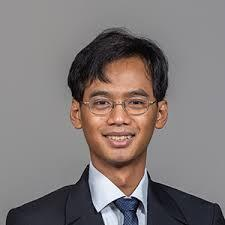
\includegraphics[width=\linewidth]{prof.jpg}
    pls give me A+ prof thanks
\end{center}

\end{multicols*}

\end{document}